\clearpage
\section{Modelo de Datos}

\subsection{Justificación}
Para la aplicación final, se hará uso de un modelo de base de datos orientado a grafos. También se contará con un esquema perteneciente a la categoria NoSQL.
 Las características de una base de datos NoSQL son las siguientes: 

\begin{itemize}
  \item Modelo de datos flexible.
  \item Buen rendimiento en clusters.
  \item Sin esquemas.
\end{itemize}

Este tipo de bases resultan útiles debido a que se se pretende procesar grandes volúmenes de información.

Las tecnologías para grandes volumenes de información son relativamente nuevas; estas surgieron debido a la necesidad que tenían empresas grandes como Google y Amazon.

La información fue convertida de un modelo relacional a un modelo basado en documentos, jerárquico o basado en columnas usando proceso de denormalización, ésto con la finalidad de dar un orden a la información considerando simplemente consultas de cierto tipo evitando así operaciones típicas del álgebra relacional cómo el Producto Cartesiano, que implicaba el uso de grandes recursos.

Las tecnologías de tipo NoSQL se orientan a consultas y no a transacción. Lo que brinda un fácil acceso a la información, una estructura de los datos orientada a su posterior análisis, respuestas en tiempo real y una gran capacidad de escalar y replicar.

Empresas cómo Foursquare, Google, Amazon, Uber o Twitter, han optado por complementar la información que persisten de forma relacional con modelos orientados a documentos usando tecnologías como Hbase, MongoDB, BigTable, DynamoDB, por citar algunos ejemplos.

\subsection{Descripción}

Para la API, el problema fundamental recae en que las recomendaciones pueden ser utilizadas para diversos casos de estudio, buscando una generalización de las características mínimas requeridas para realizar recomendaciones se plantea un modelo de datos utilizando tres principales entidades: Usuarios, Articulos a recomendar, y Categorias como características que permitan clasificar los diferentes artículos. La información que será guardada y posteriormente consultada por otros módulos del sistema seguirá un esquema propuesto por el equipo de trabajo, éste recopila la estructura de evaluaciones básicas generadas en practicamente cualquier tipo de articulos, peliculas, platillos, libros, entre otros como podemos ver en diagrama de grafos de la figura~\ref{fig:min model}.

\newpage
    \begin{landscape}
      \begin{figure}[h!]
      \centering
      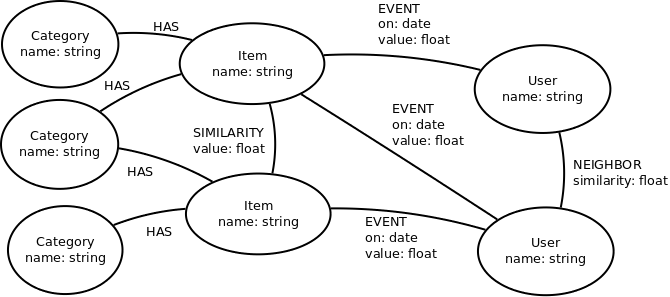
\includegraphics[width=22.5cm,height=12cm]{./images/general_data_model.png}
      \caption{Modelo general necesario para el manejo de la información}
      \label{fig:min model}
    \end{figure}
    \end{landscape}
  \newpage
